\title{Maths Stats Formulas and Definitions}
\author{ Boyd Kane }
\date{\today}
\documentclass[12pt]{article}
% Allow images to be used
\usepackage{graphicx}
\graphicspath{{./images/}}
% Clickable hyperlinks
\usepackage{hyperref}
% Colourful equations
\usepackage[dvipsnames]{xcolor} 
% Nice math
\usepackage{amsmath} 
% Nice symbols in math
\usepackage{amssymb} 
% Make the independance symbol with two perperndiculars next to each other
\newcommand{\indep}{\perp \!\!\! \perp}

\begin{document}
\maketitle
\tableofcontents
\section{Common Distributions}
\subsection{Poisson Distribution}
\begin{equation*}
    \begin{aligned}
        X &\sim Poi(\lambda) \qquad\\
        \mathbb{E}[X] &= \lambda \\
        \mathbb{V}[X] &= \lambda \\
    \end{aligned}
    \begin{aligned}
        f_X(x) &= \frac{\lambda^x e^{-\lambda}}{x!} \\
        \mathbb{E}[s^X] &= e^{\lambda \left(e^s - 1\right)} \\
        \left(\sum_{i=0}^nPoi(\lambda_i) \right) &\sim Poi \left(\sum_{i=0}^n \lambda_i \right)\\
    \end{aligned}
\end{equation*}

\subsection{Negative Binomial Distribution}
\begin{equation*}
    \begin{aligned}
        X &\sim NegBin(p, r) \qquad\\
        \mathbb{E}[X] &= \frac{r}{p} \\
        \mathbb{V}[X] &= \frac{rq}{p^2} \\
    \end{aligned}
    \begin{aligned}
        f_X(x) &= \binom{k-1}{r-1}p^rq^{k-r} \\
        \mathbb{E}[e^{sX}] &= \left(\frac{pe^s}{1 - qe^s}\right)^r \\
    \end{aligned}
\end{equation*}

\subsection{Geometric Distribution}
\begin{equation*}
    \begin{aligned}
        X &\sim Geo(p) \qquad\\
        \mathbb{E}[X] &= \frac{1}{p} \\
        \mathbb{V}[X] &= \frac{q}{p^2} \\
    \end{aligned}
    \begin{aligned}
        f_X(x) &= pq^{x-1}              \\
        \mathbb{E}[e^{sX}] &= \frac{e^tp}{1 - e^tq} \\
    \end{aligned}
\end{equation*}

\subsection{Binomial Distribution}
\begin{equation*}
    \begin{aligned}
        X &\sim Binomial(n, p) \qquad\\
        \mathbb{E}[X] &= np \\
        \mathbb{V}[X] &= npq \\
    \end{aligned}
    \begin{aligned}
        f_X(x) &= \binom{n}{x} p^x q^{n-x} \\
        \mathbb{E}[e^{sX}] &= (1 - p + pe^s)^n \\
    \end{aligned}
\end{equation*}

\subsection{Beta Distribution}
\(0 < x < 1\)
\begin{equation*}
    \begin{aligned}
        X &\sim Beta(a, b) \qquad\\
        \mathbb{E}[X] &= \frac{a}{a + b} \\
        \mathbb{V}[X] &= \frac{ab}{(a + b)^2(a + b + 1)}\\
    \end{aligned}
    \begin{aligned}
        f_X(x) &= \frac{(a + b - 1)!}{(a - 1)! (b - 1)!} \cdot x^{a-1} (1 - x)^{b-1} \\
    \end{aligned}
\end{equation*}

\subsection{Normal Distribution}
\begin{equation*}
    \begin{aligned}
        X &\sim N(\mu, \sigma^2) \qquad\\
        \mathbb{E}[X] &= \mu \\
        \mathbb{V}[X] &= \sigma^2 \\
    \end{aligned}
    \begin{aligned}
        f_X(x) &= \frac{1}{\sqrt{2\pi\sigma^2}} e^{-\frac{1}{2}\left(\frac{x - \mu}{\sigma}\right)^2} \\
        \mathbb{E}[e^{sX}] &= e^{\mu s + \frac{1}{2}s^2\sigma^2} \\
    \end{aligned}
\end{equation*}

\subsection{Gamma Distribution}
\(\lambda > 0, \alpha > 0 \)
\begin{equation*}
    \begin{aligned}
        X &\sim Gamma(\lambda, \alpha) \qquad\\
        \mathbb{E}[X] &= \frac{\alpha}{\lambda} \\
        \mathbb{V}[X] &= \frac{\alpha}{\lambda^2} \\
    \end{aligned}
    \begin{aligned}
        f_X(x) &= \frac{\lambda^\alpha x^{\alpha - 1} e^{-\lambda x}}{(\alpha - 1)!} \\
        \mathbb{E}[e^{sX}] &= \left(\frac{\lambda}{\lambda - s}\right)^\alpha \\
    \end{aligned}
\end{equation*}

\subsubsection{Notes}
Sum of independant Exponentials is Gamma distributed:
\begin{equation*}
    \left(\sum^{n} Exp(\lambda) \right) \sim Gamma(\lambda, n) 
\end{equation*}
\begin{equation*}
    Exp(\lambda) \equiv Gamma(\lambda, 1) 
\end{equation*}


\subsection{Exponential Distribution}
\begin{equation*}
    \begin{aligned}
        X &\sim Exp(\lambda) \qquad\\
        \mathbb{E}[X] &= \frac{1}{\lambda} \\
        \mathbb{V}[X] &= \frac{1}{\lambda^2} \\
        \hat{\lambda}_{MLE} &= \frac{1}{\bar{x}} \\
    \end{aligned}
    \begin{aligned}
        f_X(x) &= \lambda e^{-\lambda x} \quad x \ge 0, \lambda > 0 \\
        F_X(x) &= 1 - e^{-\lambda x} \\
        \mathbb{E}[e^{sX}] &= \frac{\lambda}{\lambda - s} \quad s < \lambda \\
        \mathbb{P}[Exp(\lambda_1) < Exp(\lambda_2)] &= \frac{\lambda_1}{\lambda_1 + \lambda_2}\\
    \end{aligned}
\end{equation*}

\subsection{Chi-Squared Distribution}
Work in progress
\section{Generating Functions}
\subsection{Probability Generating Functions}
\begin{equation*}
    \begin{aligned}
        \mathbb{G}_X(s) :&= \mathbb{E}[s^X] \\
                         &= \sum_{x = 0}^\infty s^x \cdot f_X(x) \\
        \mathbb{G}_X(0)  &= f_X(0) = \mathbb{P}[X=0] \\
        \mathbb{G}_X(1)  &= \sum_{x = 0}^\infty 1^x \cdot f_X(x) \\
                         &= 1 \\
        \mathbb{E}[X] &= \mathbb{G}_X'(1)  \\
        \mathbb{V}[X] &= \mathbb{G}_X''(1) + \mathbb{G}_X'(1) - \left(\mathbb{G}_X'(1)\right)^2 \\
    \end{aligned}
\end{equation*}


\subsection{Moment Generating Functions}
Work in progress.
\section{Infinite Sums}
Work in progress.
\section{3041F: Chains}
\subsection{Chapman-Kolmogorov Equations}
Basically, for Markov chains we can just do matrix multiplication to go from time \(i\) to time \(i + 1\).
For \(0 \le v \le t\), and \(p_{ij}(s, t) := \mathbb{P}[X_{s+t} = j | X_s = i]\):
\begin{equation*}
    p_{ij}(s, t) = \mathbb{P}[X_{s+t} = j | X_s = i] = 
    \sum_{k \in \mathcal{U}}p_{ik}(s, v) \cdot p_{kj}(s + v, t - v)
\end{equation*}

Or, in matrix notation:

\begin{equation*}
    \mathbf{P}^{(t)}(s) = \mathbf{P}^{(v)}(s) \cdot \mathbf{P}^{(t-v)}(s + v)
\end{equation*}
And under time homogeneity
\begin{equation*}
    \mathbf{P}^{(t)} = \mathbf{P}^{v} \cdot \mathbf{P}^{t-v} = \mathbf{P}^{t} 
\end{equation*}
\section{3041F: Branching Processes}
Let \(Z_m\) be the number of individuals in Generation \(m\).
Let \(X_{im}\) be the number of offspring produced by individual \(i\) in generation \(m\).
Assume all \(X_{im} = X\), so all \(X_{im}\) are identically distributed.
Assume \(Z_0 = 1\) which implies \(Z_1 = X\).

\begin{equation*}
    \mathbb{E}[Z_m] = \mathbb{E}[X]^m
\end{equation*}

Let \(\mu =\mathbb{E}[X]\) and \(\sigma^2 = \mathbb{V}[X]\).

\begin{equation*}
    \mathbb{V}[Z_m] = m\sigma^2 \qquad \text{if} \, \mu = 1
\end{equation*}
\begin{equation*}
    \mathbb{V}[Z_m] = \sigma^2 \cdot \mu^{m-1} \left( \frac{\mu^{m} - 1}{\mu - 1} \right) \qquad \text{if}\, \mu \ne 1
\end{equation*}
\section{3041F: Probability of Extinction}
To calculate the probability that the process is extinct by generation m:
\begin{equation*}
    \mathbb{P}[\text{Extinction by generation } m] = \mathbb{P}[Z_m = 0] = \mathbb{G}_m(0)
\end{equation*}

But to calculate the probability that the process is extinct at exactly generation m:
\begin{equation*}
    \mathbb{P}[\text{Extinction at generation } m] = \mathbb{G}_m(0) - \mathbb{G}_{m-1}(0)
\end{equation*}

Define the probability of extinction:
\begin{equation*}
    \begin{aligned}
        \eta :&= \mathbb{P}[\text{Eventual Extinction}] = \mathbb{P}\left[\bigcup_{m=1}^{\infty} \{ Z_m = 0 \}\right] \\
              &= \text{smallest non-negative integer root of } \mathbb{G}_X(s) = s \\
    \end{aligned}
\end{equation*}
\section{3041F: First Passage Probabilities}
\begin{equation*}
    \begin{aligned}
        p_{ij}^{(n)} :&= \mathbb{P}[X_{t+n} = j | X_{t} = i]  \\
        P &= \left[ p_{ij}\right]\\
        P_{ij}(s) :&= \sum_{n=0}^{\infty} p_{ij}^{(n)} \cdot s^n \\
        \mathbf{P}(s) :&= \left[ P_{ij}(s) \right]\\
                       &= \left( \mathbf{I} - s \cdot P \right)^{-1}\\
                       &= \left( \mathbf{I} - s \cdot \left[ p_{ij}\right] \right)^{-1}\\
        f_{ij}^{(k)} &= \mathbb{P}[\text{a k-step passage from i to j}] \qquad f_{ij}^{(0)} = 0 \,\forall\, i, j \\
        F_{ij}(s) &= \sum_{n=0}^{\infty} f_{ij}^{(n)} \cdot s^n \\
    \end{aligned}
\end{equation*}

Don't forget the test comes with identities for converting Probability matrices to first return probabilities.
\section{3041F: Discrete Time}
\subsection{Calculating the Count at a given Time}
\subsubsection{Forecasting}
\begin{equation}
    \mathbb{P}[N_{n+k} = a + i | N_n = a] = 
    \binom{k}{i} \cdot p^i \cdot q^{k-i}
\end{equation}

\begin{equation}
    (N_{n+k} - N_n) \sim Binomial(k, p)
\end{equation}

\begin{equation}
    (N_{n+k} - N_n) \indep N_n
\end{equation}

\begin{equation}
    \mathbb{E}[N_{n+k} | N_n = a] = k \cdot p + a
\end{equation}

\begin{equation}
    \mathbb{V}[N_{n+k} | N_n = a] = k \cdot p \cdot a
\end{equation}

\subsubsection{Backcasting}
\begin{equation}
    \mathbb{P}[N_n = a | N_{n+k} = a + i] = 
    \frac{
        \binom{n}{a} \binom{k}{i}
        }{
        \binom{n+k}{a+i}
    }
\end{equation}
\begin{equation}
    \mathbb{P}[N_n = a | N_{n+k} = a + i] \sim HyperGeo(n+k, n, a+i)
\end{equation}

\begin{equation}
    \mathbb{E}[N_n | N_{n+k} = a + i] = \frac{(a + i) \cdot n}{n + k}
\end{equation}

\begin{equation}
    \mathbb{V}[N_n | N_{n+k} = a + i] = 
    \frac{n + k - a - i}{n + k - 1} \cdot 
    \frac{(a + i) \cdot n}{ n + k} \cdot 
    ( 1 - \frac{n}{n + k})
\end{equation}

\subsection{Calculating the Time until a given Count}
\begin{equation}
    T_a \sim NegBinomial(a, p) 
\end{equation}

\begin{equation}
    \mathbb{E}[T_a] = \frac{a}{p}
\end{equation}

\begin{equation}
    \mathbb{V}[T_a] = \frac{a \cdot q}{p^2}
\end{equation}


\subsubsection{Forecasting}
\begin{equation}
    \mathbb{P}[T_{a + i} = t + j | T_a = t] =
    \binom{j-1}{i-1} \cdot p^i \cdot q^{j-i}
\end{equation}

\begin{equation}
    \mathbb{P}[T_{a + i} = t + j | T_a = t] \sim NegBinomial(i, p)
\end{equation}


\begin{equation}
    \mathbb{P}[T_{a + i} | T_a = t] = 
    \frac{i}{p} + t
\end{equation}

\begin{equation}
    \mathbb{P}[T_{a + i} | T_a = t] = 
    \frac{i \cdot q}{p^2}
\end{equation}

\subsubsection{Backcasting}
\begin{equation}
    \mathbb{P}[T_a = t | T_{a + i} = t + j] =
    \frac{
        \binom{t - 1}{a - 1} \cdot \binom{j - 1}{i - 1}
        }{
        \binom{t + j - 1}{a + i - 1}
    }
\end{equation}

\begin{equation}
    \mathbb{E}[T_a | T_{a + i} = t + j] = \frac{a (t + j)}{ a + i }
\end{equation}


\begin{equation}
    \mathbb{V}[T_a | T_{a + i} = t + j] = 
    \frac{
        a i (t + j) (t + j - a - i)
        }{
        (a + i)^2 (a + i + 1)
    }
\end{equation}
\section{3041F: Continuous Time}
With the assumptions that \(\lambda_i = \lambda\) and \(t_i = t\) for all i:

\begin{equation}
    X_i \sim Poisson(\lambda t)
\end{equation}

\begin{equation}
    Y_n = \sum_{i = 1}^{n} X_i
\end{equation}

\begin{equation}
    Y_n \sim Poisson(n \lambda t)
\end{equation}

\begin{equation}
    Y_{n+k} - Y_n \sim Poisson(k \lambda t)
\end{equation}

\begin{equation}
    \mathbb{C}ov[Y_n, Y_m] = \lambda \cdot t \cdot min(n, m)
\end{equation}

\begin{equation}
    \mathbb{C}orr[Y_n, Y_m] = \frac{min(n, m)}{\sqrt{nm}}
\end{equation}

\subsection{Calculating the Count at a given Time}
\subsubsection{Forecasting}
\begin{equation}
    \mathbb{P}[Y_{n + k} = a + i | Y_n = a] =
    \frac{
        e^{-k \lambda t} \cdot (k \lambda t)^i
    }{ i! }
\end{equation}

\begin{equation}
    \mathbb{E}[Y_{n + k} | Y_n = a] = k \lambda t + a
\end{equation}

\begin{equation}
    \mathbb{V}[Y_{n + k} | Y_n = a] = k \lambda t
\end{equation}

\subsubsection{Backcasting}
\begin{equation}
    \mathbb{P}[Y_n = a | Y_{n + k} = a + i ] =
    \binom{a + i}{a} 
    \left(\frac{n}{n + k}\right)^a 
    \left(\frac{k}{n + k}\right)^i
\end{equation}

\begin{equation}
    \mathbb{P}[Y_n = a | Y_{n + k} = a + i ] 
    \sim Binomial\left(a + i, \frac{n}{n+k}\right)
\end{equation}

\begin{equation}
    \mathbb{E}[Y_n | Y_{n + k} = a + i ] =
    \frac{(a + i) \cdot n}{n+k}
\end{equation}

\begin{equation}
    \mathbb{V}[Y_n | Y_{n + k} = a + i ] = 
    \frac{(a + i) \cdot n \cdot k}{(n + k)^2}
\end{equation}

\subsection{Calculating the Time until a given Count}

\begin{equation}
    T_1 \sim Exponential\left(\frac{1}{\lambda}\right)
\end{equation}

\begin{equation}
    T_a \sim Gamma(a, \lambda)
\end{equation}

\begin{equation}
    \mathbb{E}[T_a] = \frac{a}{\lambda}
\end{equation}

\begin{equation}
    \mathbb{V}[T_a] = \frac{a}{\lambda^2}
\end{equation}

\subsubsection{Forecasting}
\begin{equation}
    \mathbb{E}[T_{a + i} | T_a = t] = \frac{i}{\lambda} + t
\end{equation}

\begin{equation}
    \mathbb{V}[T_{a + i} | T_a = t] = \frac{i}{\lambda^2}
\end{equation}


\subsubsection{Backcasting}
\begin{equation}
    \mathbb{E}[T_a | T_{a + i} = t + j] = \frac{a(t + j)}{a + i}
\end{equation}

\begin{equation}
    \mathbb{V}[T_a | T_{a + i} = t + j] = 
    \frac{ ai(t + j)^2 }{ (a + i)^2 \cdot (a + i + 1) }
\end{equation}
\section{3041F: Poisson Processes}
\subsection{3041F: Probability Integral Transform}
If we want a random variable, X, that should have a certain CDF, \(F_X()\),
we can take a uniform random variable \(U \sim U(0, 1)\) and 
pass it through the inverse of \(F_X()\) in order to get the random variable X:
\begin{equation*}
    F_X^{-1}(U) \text{ has CDF } F_X()
\end{equation*}


From this, the exponential distribution can be simulated as 
\begin{equation*}
    -\frac{1}{\lambda}ln(U) \sim Exp(\lambda)
\end{equation*}

And the Gamma distribution with \(n\) iid uniform random variables as:
\begin{equation*}
    -\frac{1}{\lambda}ln(U_1 \cdot U_2 \cdot \dots \cdot U_n) \sim Gamma(n, \lambda)
\end{equation*}

\subsection{3041F: Estimation}
See page 5 in the notes
\section{3041F: Basic Poisson Process}
\subsection{3041F: Poisson Postulates}
A counting process \(\{N(t), t \ge 0\}\) is a Poisson process with rate 
\( \lambda > 0 \), for small h, iff:
\begin{enumerate}
    \item N(0) = 0
    \item The process has independant and stationary increments
    \item \(\mathbb{P}[N(h) = 1] = \lambda h + o(h)\)

        So the Probability of one occurance within small timeframe h is equal to the rate parameter times h, plus some terms that go to zero.
    \item \(\mathbb{P}[N(h) > 1] = o(h)\)

        So the Probability of more than one occurance within small timeframe h goes to zero.
\end{enumerate}

\subsection{Poisson Process Information}
Proof page 7 in the notes.

The number of events in an interval of length t for a Poisson process with 
rate parameter \(\lambda\) is a random variable distributed \(Poi(\lambda t)\).

More explicitly, for n a non-negative integer:
\begin{equation*}
    \mathbb{P}[N(t) = n] = \frac{e^{-\lambda t}(\lambda t)^n}{n!}
\end{equation*}

The interarrival times \({T_n, n=1, 2, \dots}\) are iid \(\sim Exp(\lambda)\)

Define the sequence of waiting times \({S_n, n=1, 2, \dots}\) as: 
\begin{equation*}
    \left(S_n := \sum_{i=1}^n T_i\right) \sim Gamma(n, \lambda)
\end{equation*}


The sequence of arrival times \({S_i, i=1, 2, \dots, n}\) have the same distribution as an ordered sample of size \(n\) taken from \(U(0, S_n)\)


If we have a Poisson process \(\{N(t), t \ge 0\}\) where we classify each event as type 1
with probability \(p\) and type 2 with probability \(1-p\), then 
\(\{N_1(t), t \ge 0\}\) and \(\{N_2(t), t \ge 0\}\) are independant Poisson 
processes with parameters \(\lambda p\) and \(\lambda (1-p)\)


Let \(\{N^{(1)}(t), t \ge 0\}\) and \(\{N^{(2)}(t), t \ge 0\}\) be independant Poisson 
Processes with rates \(\lambda_1\) and \(\lambda_2\).
Also define the arrival times \(S^{(1)}_n\) and \(S^{(2)}_m\) as the arrival of the nth, mth event.

Then:
\begin{equation*}
    \mathbb{P}[S^{(1)}_n < S^{(2)}_m] = 
    \sum_{i=n}^{n + m - 1} 
    \binom{n + m - 1}{i} 
    \left( \frac{\lambda_1}{\lambda_1 + \lambda_2} \right)^i 
    \left( \frac{\lambda_2}{\lambda_1 + \lambda_2} \right)^{n + m - 1 - i}
\end{equation*}
\subsection{3041F: Modelling Poisson Processes}
There are two forms for modelling a Poisson process. 
Either you decide on how many events you want and let the events dictate the timeframe,
or you decide on the timeframe you want and take note of the events in that timeframe.

\paragraph{Generating n events} Calculate the events by sampling from a uniform distribution and then calculating \(T_i = -\frac{1}{\lambda} ln(U_i(0,  1))\) for \(i = 1, \dots, n\). 
\paragraph{Generating events in timeframe} Define the interarrival times as \(T_1, \dots, 
T_N\) where all interarrival times are in the interval \([0, T]\)
\subsection{3041F: Estimation of Poisson Processes}
Again, there are two scenarios. Either generate n events, or generate events within a timeframe \([0, t]\).

If the first n events of a process are observed as the interarrival times \(t_i, \dots, t_n\). Then the MLE of \(\lambda\) is:
\begin{equation*}
    \hat{\lambda}_{MLE} = \frac{n}{\sum_{i=1}^{n}t_i}
\end{equation*}


Alternatively, if there are N observed events in a given time interval \([0, T]\), then the MLE doesn't depend on the observed interarrival times and is:
\begin{equation*}
    \hat{\lambda}_{MLE} = \frac{N}{T}
\end{equation*}
Also, since \(N \sim Poi(\lambda T)\), \(\hat{\lambda}_{MLE}\) is an unbiased estimate of 
\(\lambda\) with variance \(\frac{\lambda}{T}\).
\section{3041F: Compound Poisson Processes}
For regular poisson processes, every event is identical and increases the count by a 
certain amount. The events themselves aren't random, it's only the duration inbetween
events which is random.

For Compound Poisson Processes, both the duration between events, and the amount by 
which our count will be changed is a random variable.

Let \(X_1, \dots X_N\) be a sequence of iid random variables with PFG \(P_X(s)\) and N a non-negative integer valued random variable with PGF \(P_N(s)\).

Then the count \(S_N\) and the PGF thereof are:
\begin{equation*}
    \begin{aligned}
        S_N &= \sum_{i=1}^{N} X_i \\
        P_{S_N}(s) &= P_N(P_X(s)) \\
    \end{aligned}
\end{equation*}
The Expectation and Variance of \(S_N\) are given as a corollary:
\begin{equation*}
    \begin{aligned}
        \mathbb{E}[S_N] &= \mathbb{E}[N] \mathbb{E}[X]\\
        \mathbb{V}[S_N] &= \mathbb{E}[N]\mathbb{V}[X] + \left( \mathbb{E}[X]\right)^2 \mathbb{V}[N]\\
    \end{aligned}
\end{equation*}


We formally define a compound Poisson process as a stochastic 
process \(\{X(t), t > 0\}\) that can be represented as the sum of iid random variables \(X_i\) which are also independant of the Poisson process:
\begin{equation*}
    X(t) = \sum_{i = 1}^{N(t)} X_i
\end{equation*}

From this we can give the moments for a compound poisson process. With \(X(t)\) as the 
compound poisson process made up of the random variables \(X_i: i=1, 2, \dots\):
\begin{equation*}
    \begin{aligned}
        \mathbb{E}[X(t)] &= \lambda t \mathbb{E}[X]   \\
        \mathbb{V}[X(t)] &= \lambda t \mathbb{E}[X^2] \\
    \end{aligned}
\end{equation*}
\section{3041F: Non-homogeneous Poisson Processes}
Regular Poisson Processes don't care what time it is. 
The rate parameter \(\lambda\) is constant, it doesn't change. This means that the frequency of events is constant.
Non-homogeneous Poisson processes replace the constant rate parameter \(\lambda\) with a function that depends on the time, called the intensity function \(\lambda(t)\).

The non-homogeneous poisson postulates have to be rephrased slightly:

A counting process \(\{N(t), t \ge 0\}\) is a Poisson process with intensity function
\( \lambda(t) > 0 \) and \(t > 0 \) for small h, iff:
\begin{enumerate}
    \item N(0) = 0
    \item The process has independant increments (we drop the requirement for stationary increments)
    \item \(\mathbb{P}[N(t + h) - N(t) = 1] = \lambda(t) h + o(h)\)

        So the Probability of one occurance within small timeframe t to t + h is equal to the intensity( at time t) multiplied by h, plus some terms that go to zero.
    \item \(\mathbb{P}[N(t + h) - N(t) > 1] = o(h)\)

        So the Probability of more than one occurrence within small timeframe from t to t + h goes to zero.
\end{enumerate}
\subsection{3041F: Mean Value Function}
Define the mean value function m(t) the integral from 0 to t of \(\lambda(t)\):
\begin{equation*}
    m(t) = \int_{0}^{t} \lambda(u) \, du
\end{equation*}
And then the number of events in a time interval (t, t + s] for a non-homogeneous Poisson 
process is \(\sim Poi({\color{BrickRed}{m(t + s) - m(t)}})\), with 
colours added to make it clear that \({\color{BrickRed}{m(t + s) - m(t)}}\) is just the 
rate parameter to a Poisson distribution.


In English, the number of events over a given interval is poisson 
distributed with a rate proportional to the total intensity over that interval. So the probability looks like:
\begin{equation*}
    \begin{aligned}
        \mathbb{P}[N(t + s) - N(t) = n] &= \frac{
            e^{-\left({\color{BrickRed}{m(t+s) - m(t)}}\right)} 
            \cdot \left( {\color{BrickRed}{m(t+s) - m(t)}}\right)^n
        }{n!} \\
        \end{aligned}
    \end{equation*}
    \subsection{3041F: Simulation of a non-homogeneous Poisson Process}
    Suppose that events arrive according to a poisson process with rate \(\lambda\), but we only consider some of the events, choosing events with probability p(t).\newline \newline

    This describes a non-homogeneous Poisson process with intensity function \(\lambda(t) = \lambda \cdot p(t)\). 
    We can therefore simulate a non-homogeneous Poisson process by first using our methods for homogeneous poisson processes, and then discarding events according to the probability function p(t).  \newline \newline

    \subsubsection{The Thinning algorithm}
    The thinning algorithm generates a non-homogeneous poisson process by finding an constant valued 
    approximation of the rate function, generating a homogeneous poisson process according to this 
    constant, and then discarding some events such that the approximation of the rate function 
    becomes the actual rate function.

    If we want to simulate over a time interval [0, T] according to intensity function 
    \(\lambda(t) > 0\) first generate events according to a poisson process with rate \(\lambda\)
    over the interval [0, T] to give the N interarrival times \(T_1, \dots, T_N\).\newline
    Then select \(\lambda_{max}\) such that 
    \begin{equation*}
        \lambda_{max} \ge \lambda(t) \qquad \forall \, t \in [0, T]
    \end{equation*}

    Finally, create an indicator function with \(\lambda_{max}\) to select only those events where
    a Uniform random variable in the range [0, \(\lambda_{max}\)) is less than \(\lambda(t)\): 
    \begin{equation*}
        U(0, \lambda_{max}) \le \lambda(t) \quad \text{for } t = \sum_{i=1}^{j} T_i
    \end{equation*}

    Then all those selected events make up the required non-homogeneous poisson process.
    \subsubsection{Subintervals for simulations}
    The thinning algorithm will regect lots of events if the intensity function \(\lambda(t)\) 
    is very different from \(\lambda_{max}\). We can fix this by dividing up the time interval
    into multiple smaller subintervals, and then running the thinning algorithm individually on
    each of these sub-intervals. Each time calculating a new and different value for 
    \(\lambda_{max}\).
    \subsubsection{Combining homogeneous Poisson Processes}
    Since the sum of events for two independant Poisson Processes with rates 
    \(\lambda_1\) and \(\lambda_2\) is itself a Poisson Process with rate \(\lambda_1 + \lambda_2\)
    we can use this to efficiently create piecewise Poisson processes where the 
    intensity function \(\lambda(t)\) is sometimes constant.
    \subsection{3041F: Estimation of non-homogeneous Poisson Processess}
    The PDf of the ith interarrival time given the waiting time of the (i-1)th can be written as:

    \begin{equation*}
        f_{T_i | W_{i-1}}(t) = 
        \lambda(w_{i-1} + t) \cdot e^{-\left(m(w_{i-1} + t) - m(w_{i-w})\right)}
    \end{equation*}

    Note that the arrival times are independant due to the increments being independant. \newline \newline

    Note that the probability of the ith interarrival time being greater than some value t (given 
    the (i-1)th arrival time) is equivalent to the probability of there being zero events between 
    the (i-1)th arrival time and the (i-1)th arrival time plus t. This implies:

    \begin{equation*}
        \begin{aligned}
            \mathbb{P}[T_i > t | W_{i-1} = w_{i-1}] &= \mathbb{P}[N(w_{i-1} + t) - N(w_{i-1}) = 0] \\
                                                    &=  e^{-\left(m(w_{i-1} + t) - m(w_{i-w})\right)} \\
        \end{aligned}
    \end{equation*}
    \subsubsection{Likelihood for non-homogeneous Poisson Processes}
    In general, explicit expressions for the MLEs do not exist, and likelihood maximisation must be 
    done numerically.
    The notes give examples, but they all boil down to two different cases. The first case is when we have data about the first \(n\) arrivals, and can be calculated as so:
    \begin{enumerate}
        \item taking a given intensity function with unknown parameters \(\theta\) and observed waiting times \(w_1, \dots, w_n\),
        \item Calculating the log-likelihood function as 
            \begin{equation*}
                l(\theta) = \sum_{i=1}^{n}ln\left(\lambda(w_i; \theta)\right) - 
                \left(m(w_n; \theta) - m(w_0; \theta)\right)
            \end{equation*}
        \item and then maximising \(l\) with respect to \(\theta\) in order to find the MLEs for \(\theta\).
    \end{enumerate}

    The second case is where we've measured all arrivals in an interval [0, T], and can be 
    calculated as shown below. It is different, because we need to account for the probability that 
    we saw no additional events between our last observed event and T.
    \begin{enumerate}
        \item taking a given intensity function with unknown parameters \(\theta\) and observed waiting times \(w_1, \dots, w_n\). All waiting times should be within [0, T].
        \item Calculating the likelihood function as 
            \begin{equation*}
                L(\theta) = \prod_{i=1}^{N}\lambda(w_i; \theta) e^{-m(T; \theta)}
            \end{equation*}
        \item and then maximising \(L\) with respect to \(\theta\) will give the MLEs of \(\theta\).
    \end{enumerate}

    The notes also go into likelihood ratio tests for seeing if a particular Poisson process is non-
    homogeneous, but I'm not going to write that up here.

    \section{3041F: Time Series Analysis}
    \marginpar{\href{https://media.uct.ac.za/engage/theodul/ui/core.html?ltimode=true&id=b6171c7c-14c0-46a4-aa3b-9be2aa42f87f}{Time Series Video 1}}
    This course will only look at measurements that are equally spaced in time. We will not be looking at unequal spacing (ie when you measure each event as it comes).

    A time series is denoted as \(X_t, t \, \in T\) where T can be discrete or continuous.\newline
    The index \(t\) will be discrete in this course.
    \(X_t\) could be continuous, discrete, or (not in this course) qualitative. \newline \newline

    We will often plot the data, try to see if there are any patterns or trends, and then plot summary statistics which could help with forecasting.


    There are several objectives of time series analysis:
    \begin{itemize} 
        \item Description: Summarizing the data in useful ways like expectation, variance, etc.
        \item Modelling: Creating a mathematical model of the data that closely predicts what has happened.
        \item Forecasting: Using the created model to give confidence intervals and estimates for where the process will be at a specified point in the future.  Forecasting is possible through historical data, and the existance of a pattern in that data which is expected to continue into the future.
        \item Control: Deciding if a given process is beyond certain safe operating bounds or if some extra factors need to be applied to the process in order to keep it within those safe operating bounds.
    \end{itemize} 

    \marginpar{\href{https://media.uct.ac.za/engage/theodul/ui/core.html?ltimode=true&id=97be9e42-a0d6-4a54-b08e-853b4dac6c8b}{Time Series Video 2}}
    Time series are often modelled additively as a sequence of components: 
    \begin{itemize} 
        \item Trend \(\mu_t\): The underlying expectation at time \(t\) of the time series. Often modelled as a simple function.
        \item Seasonality \(s_t\): When there are repetitions in the data, with peaks and troughs.
        \item Cycles \(c_t\): which is excluded in this course.
        \item Noise \(e_t\): which represents the random fluctuations of the data.
    \end{itemize} 
    % TODO try add a matplotlib plot instead of this
    \begin{figure}[t]
        \centering
        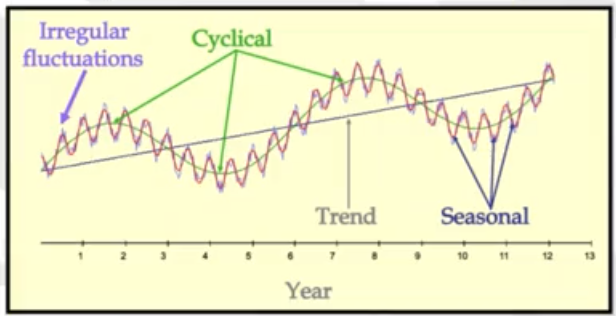
\includegraphics[width=8cm]{cycles_vs_seasons}
        \caption{Comparison of Seasons vs Cycles}
    \end{figure}

    Not every component will be included in every model.
    This can be modelled as 
    \begin{equation*}
        X_t = \mu_t + s_t + c_t + e_t
    \end{equation*}
    Or multiplicatively, although the multiplicative model will be log-transformed and then we'll just treat it as an additive model.
    \begin{equation*}
        \begin{aligned}
            X_t &= \mu_t \cdot s_t \cdot c_t \cdot e_t \\
            ln(X_t) &= ln(\mu_t) + ln(s_t) + ln(c_t) + ln(e_t) \\
        \end{aligned}
    \end{equation*}
    \subsection{Trend}
    The long term growth/decline of a time series, modelled with a simple function. Basically just the expectation.

    We can also look at the local trend, which just takes into account \(n\) prior points of the time series instead of all the data.

    Some examples of Trend:
    \begin{itemize}
        \item \(X_t = \epsilon_t\) with \(\epsilon_t \sim N(0, a)\) all iid.
            Since model's expectation \(\mu_t = \mathbb{E}[X_t] = 0\) doesn't depend on time, 
            we can use the sample mean to estimate the population mean as all samples are from the same distribution.
        \item \(X_t = t + \epsilon_t \) with \(\epsilon_t \sim N(0, a)\) all iid.
            This model's expectation \(\mu_t = \mathbb{E}[X_t] = t\) does depend on time, so the sample mean wont' be a good estimate of the true mean.
    \end{itemize}

    \subsection{Seasonality}
    When you have repeating trends in the data such as temperature increasing every summer or business flights decreasing over the weekend.

    The amplitude of the seasonality is the difference between the peaks and troughs of the data.
    This amplitude might change over time. The amplitude will affect the variance of the overall, as a high amplitude will increase the variance.

    \subsection{Cycles}
    Basically seasonality on top of the existing seasonality. If seasonality repeats every year, then cycles repeat over decades. 

    Cycles are often used to refer to less regular oscillations in the data, such as bull and bear stock market trends which are less predictable than the annual trends produced by tax deadlines and such.
    We won't be covering the cyclical component in STA3041F.

    \subsection{Transformations}
    Because of the variablity of the data, we might have to first transform the data such that our additive model is appropriate.
    Our additive model only works with data that changes linearly in time, so if the seasonality amplitude increases exponentially then we'll have to transform the data to get rid of that exponential growth.
    The family of transformations we'll be using is the Box-Cox transformations.

    \section{3041F: Transformations}
    \marginpar{\href{https://media.uct.ac.za/engage/theodul/ui/core.html?ltimode=true&id=0ab6eb00-7b9d-4895-be8a-006463cd33b0}{Time Series Video 3}}
    In figure \ref{fig:airplane_data}, you can see the seasonal component in the repeating peaks and troughs. 
    There is an upwards trend in the data and no cyclical component

    There is an increasing amount of variance as time continues as shown by how the difference between the peaks and troughs. This implies that a multiplicative model might work well.
    \begin{figure}[t]
        \centering
        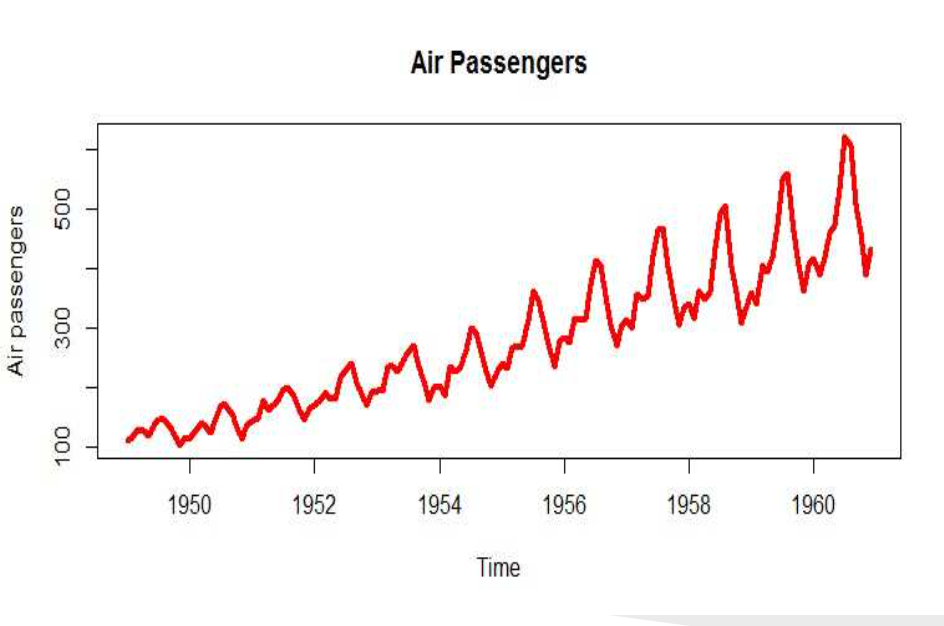
\includegraphics[width=8cm]{airplane_data}
        \caption{Airplane data}
        \label{fig:airplane_data}
    \end{figure}

    See figure \ref{fig:airplane_data_less_trend}. 
    We can now subtract the long term trend (orange) from the root data (blue) 
    in order to isolate just the error and seasonal components (assuming no 
    cyclical component):
    \begin{figure}[t]
        \centering
        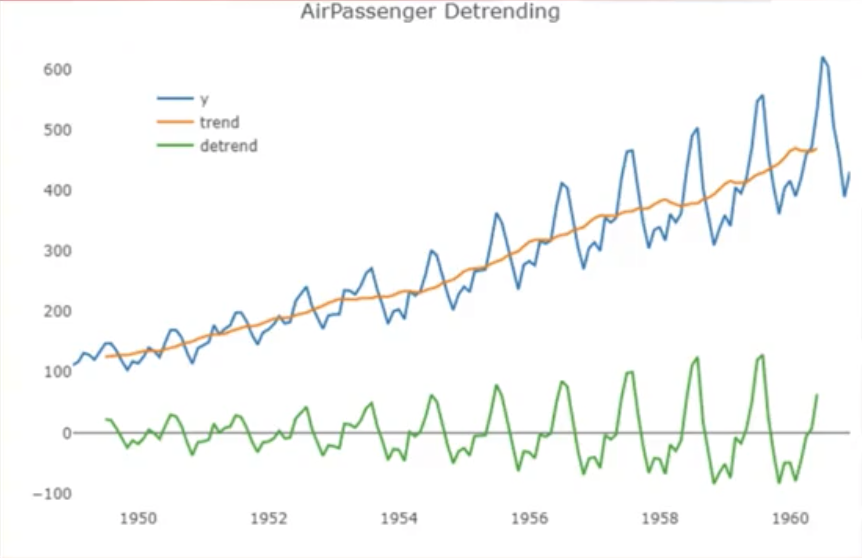
\includegraphics[width=8cm]{airplane_data_less_trend}
        \caption{Airplane data with the trend subtracted.}
        \label{fig:airplane_data_less_trend}
    \end{figure}

    Sometimes you'll want to take the root data $X_t$ and apply a transformation direcly to it
    in an attempt to end up with linear data. Transformations might also be used to make the variance equal across the series.
    Possible transformations might be $\sqrt{X_t}$, $\sqrt[3]{X_t}$, $log(X_t)$, or $-X_t^{-1}$.

    However, the Box-Cox transformation can make our lives easier:

    \subsection{3041F: Box-Cox Transformation}
    If our variance increases over time, then we want to account for this in our model. However, linear methods don't really like dealing with a changing variance. The solution is to take the original data, transform it in some way to remove/reduce how much the variance changes over time, and then proceed to use linear models on the transformed data.

    Box-Cox is a class of transformations with parameter $\lambda$  that tries to change reduce the amount the variance changes over time.

    The original series $x_1, \dots, x_n$ is transformed into $y_1(\lambda), \dots, y_n(\lambda)$ as follows:

    \begin{equation*}
        y_t(\lambda) =
        \begin{cases}
            \frac{x_t^{\lambda} - 1}{\lambda}  & \text{if $\lambda \ne 0$} \\[2ex]
            log(x_t) & \text{if $\lambda = 0$} \\
        \end{cases}
        \end{equation*}

        Where $\lambda$ has to be estimated, and the resulting transformed data has a more stabilizer variance. 
        \marginpar{\href{https://www.desmos.com/calculator/rnpu3y6lxk}{Desmos Interactive graph of the $\lambda \ne 0$ part of Box-Cox}}
        The larger value of $\lambda$, the stronger the suppressing effect of the transformation.
        Note that taking the limit as $\lambda$ trends to zero results in $log(x_t)$, which is where
        the second case of the piecewise Box-Cox comes in.
        % TODO add some matplotlib graphs showing the effect of different values of lambda

        Note that the Box-Cox tranformation is equivalent to many others, depending on the value of $\lambda$:
        \begin{itemize}
            \item When $\lambda = -1$: Inverse tranformation
            \item When $\lambda = 0$: Natural Log transformation.
            \item When $\lambda = \frac{1}{2}$: (basically) Square root transformation.
            \item When $\lambda = \frac{1}{3}$: (basically) Cube root transformation.
            \item When $\lambda = 1$: (basically) No transformation.
        \end{itemize}

        % TODO include notes on the application of Box-Cox


        \subsection{3041F: Fitting Linear Filters}
        \marginpar{\href{https://media.uct.ac.za/engage/theodul/ui/core.html?ltimode=true&id=eb6c2126-53cd-484c-a148-4cac57e904f2}{Time Series Video 4}}
        In time series analysis, we often need to remove the noise present in the data.
        Filtering the data is the processes of removing noise from the data, and there are different methods of filtering.
        \begin{figure}[t]
            \centering
            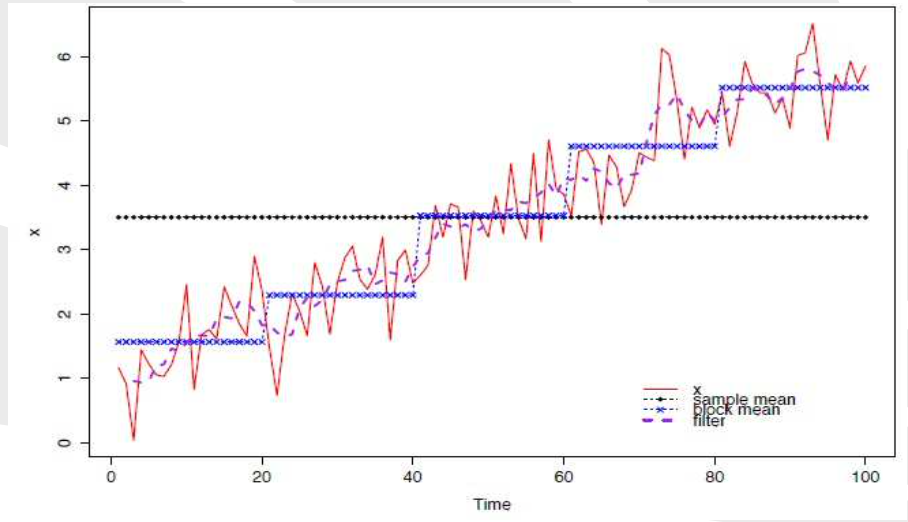
\includegraphics[width=8cm]{filtering_local_trends}
            \caption{An example of moving average, block mean, and sample mean estimates of
            the trend of the data.}
            \label{fig:filtering_local_trends}
        \end{figure}

        The sample mean of the data is often used to estimate the trend of that data. Although this assumes that the trend does not change over time (ie it's not good for increasing/decreasing data).
        An example of the sample mean is shown with the black +'s in Figure \ref{fig:filtering_local_trends}.

        A better way of estimating the trend is to divide the data into smaller blocks, and calculate the sample mean for each of those blocks. Then use these sample means to be the trend, although this still isn't great.
        An example of the block mean is shown with the blue x's in Figure \ref{fig:filtering_local_trends}.

        An even better way is via linear filters, one of which is the weighted average, an example of which is shown with the purple dashed line in Figure \ref{fig:filtering_local_trends} (labelled 'filter').

        You can see that the weighted average stays the closest to the data, while still 
        ignoring some of the jagged peaks. You can think of it as smoothing the data while
        remaining close to it.

        Linear filters can also be used to estimate seasonal components by varying various parameters that the filters take. These parameters change how smooth the filter makes the data, or how much attention it pays to local changes compared to larger scale changes.

        We can transform our original time series data $y_1, \dots, y_n$ to a filtered
        version $\tilde{y_1}, \dots, \tilde{y_n}$ by iterating over some of the items
        in $y$ and multiplying them by a weight $w$. 

        We'll look at all the $q$ items before the $y_i$ we care about, as well as all the $s$
        items after that same $y_i$. Then we'll multiply them by a weight $w_i$ and add them
        up:

        \begin{equation*}
            \tilde{y_t} = \sum_{i = -q}^{s} w_i \cdot y_{t+i}
        \end{equation*}

        Note that the $w_i$'s all have to sum to 1 (so the sample mean stays the same), 
        and usually we set $s = q$ (so we look at the same number of items behind us 
        as we do ahead of us).

        We can also show that if $\mathbb{E}[y_t] = \alpha + \beta t$ then the linear filter
        preserves this and $\mathbb{E}[\tilde{y_t}] = \alpha + \beta t$.


        The linear filter won't always preserve a quadratic trend unless we get funky with
        how we choose our weights. For example, if we have an equation for $y_t$ in the
        form:

        \begin{equation*}
            y_t = \alpha + \beta t + \phi t^2 + e_t
        \end{equation*}
        Then the expectation of our linear filter version of $y_t$ is given by
        \begin{equation*}
            \mathbb{E}[\tilde{y_t}] = \alpha + \beta t + \phi t^2 + \phi \sum_i w_i i^2
        \end{equation*}
        So in order to preserve a quadratic trend, we'd need to choose the weights $w_i$ such
        that the final term is equal to zero, ie:
        \begin{equation*}
            0 = \sum_i w_i i^2
        \end{equation*}


        Estimating the weights of the linear filter can be done as follows:
        \begin{enumerate} 
            \item Decide on how many weights you'll use. This is called the window size
            \item Decide if you're trend equation is linear, quadratic, cubic, etc.
            \item Estimate the coefficients of the trend equation $y_t = \alpha + \beta t + \dots$ using least squares.
            \item We can center the window such that the current $y_t$ is at zero, which simplifies the calculations a bit.
        \end{enumerate} 

        \paragraph{Time Series Video 5} This video was a lot of math walk-through, which I'm not going to bother writing down.
        \marginpar{\href{https://media.uct.ac.za/engage/theodul/ui/core.html?ltimode=true&id=108de531-9917-45ef-896c-90539a3e3604}{Time Series Video 5}}


        \subsection{3041F: Moving Averages}
        \marginpar{\href{https://media.uct.ac.za/engage/theodul/ui/core.html?ltimode=true&id=35c75f6e-6cf9-4e24-8a0c-1b5e9e712892}{Time Series Video 6}}
        A moving averages is a linear combination of current and past error terms.
        So we can define the moving average at time $t$ a$x_t = e_{t-n} + \dots + e_t$, 
        where we call $n$ the order of the moving average, often written as MA(n).

        There are certain useful properties, but in order for them to hold we need
        the time series to not have a seasonal component and be represented by
        \begin{equation*}
            y_t = \mu_t + e_t \qquad \text{where $\mu_t$ is the mean at time t}
        \end{equation*}
        and the error terms $e_t \sim N(0, \sigma^2)$ are all independent.
        Also, define the smoothened trend at time $t$, $\mu_t$ as:
        \begin{equation*}
            \hat{\mu}_t = \sum_{i = -s}^s w_i \cdot y_{t + i}
        \end{equation*}

        Then the following properties hold:
        \begin{equation*}
            \mathbb{V}[\hat{\mu}_t] = \sigma^2 \sum_{i = -s}^{s} w^2_i
        \end{equation*}
        \begin{equation*}
            \mathbb{C}ov[\hat{\mu}_t, \hat{\mu}_{t+k}] = 
            \sigma^2 \sum_{i = -s}^{s-k} w_i \cdot w_{i+k}
        \end{equation*}
        \begin{equation*}
            \begin{aligned}
                \mathbb{C}orr[\hat{\mu}_t, \hat{\mu}_{t+k}] &= 
                \frac{\mathbb{C}ov[\hat{\mu}_t, \hat{\mu}_{t+k}]}{
                \mathbb{V}[\hat{\mu}_t, \hat{\mu}_{t+k}]} \\
                                                            &= \frac{
                                                                \sum_{i = -s}^{s-k} w_i \cdot w_{i+k}
                                                                }{ 
                                                                \sum_{i = -s}^{s} w^2_i
                                                            }\\
                                                        \end{aligned}
    \end{equation*}

    It can also be proven that the variance of the moving average is less than the 
    variance of the original data.

    If we have a time series described by $y_t = \mu_t + e_t$ and the estimate
    for the trend is given by $\tilde{y_t}$, then we define the de-trended series
    as the difference $y_t - \tilde{y_t}$. If $\tilde{y}_t$ is an unbiased estimate
    of the trend then $\mathbb{E}[y_t - \tilde{y_t}] = 0$.

    An example of the original series and the de-trended series is shown in figure
    \ref{fig:detrended_series}

    \begin{figure}[t]
        \centering
        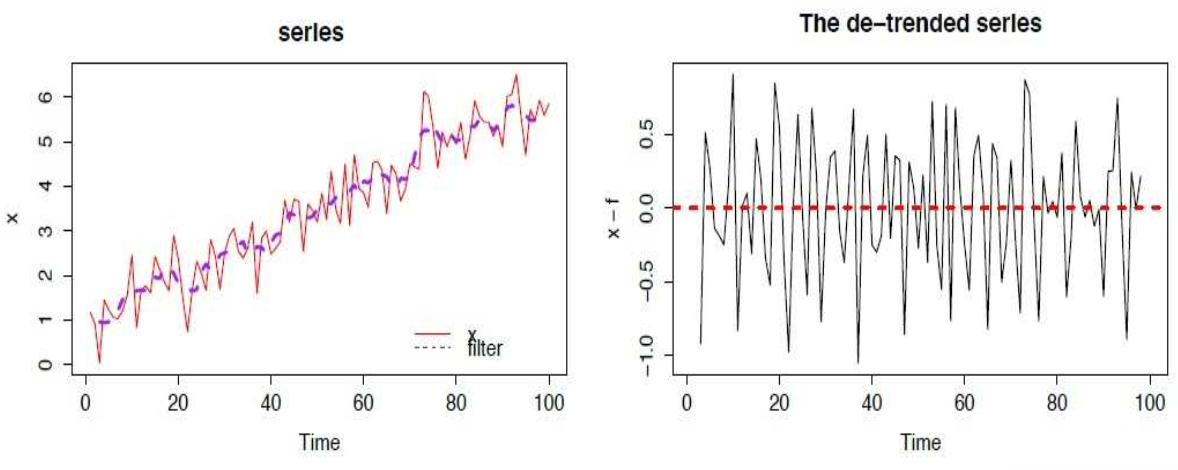
\includegraphics[width=8cm]{detrended_series}
        \caption{The detrended series has an expectation of zero if the estimate of
        the trend is unbiased.}
        \label{fig:detrended_series}
    \end{figure}

    Note that the seasonal component of a series can be removed using a moving
    average with a window size equal to the period of the season. This can be 
    seen by looking at the MA(12) line in figure \ref{fig:removing_the_seasons}


    \begin{figure}[t]
        \centering
        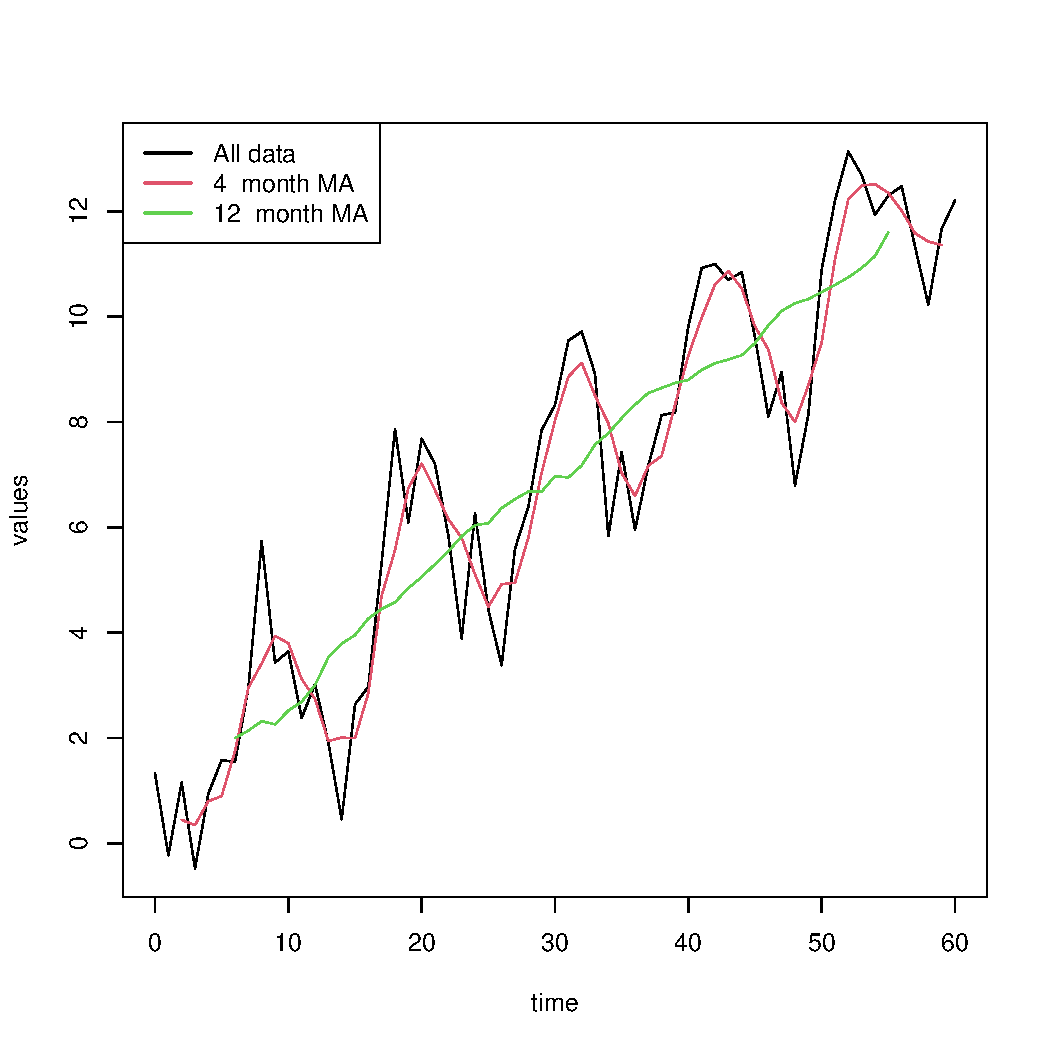
\includegraphics[width=8cm]{removing_the_seasons}
        \caption{The seasonality can be removed by applying a moving average
        which has a window size of the period of the data.}
        \label{fig:removing_the_seasons}
    \end{figure}


    Some comments about Moving Averages
    \begin{itemize} 
        \item They smoothen out a time series (ie they reduce variation)
        \item They estimate the trend of a time series
        \item The transformed series will be correlated with itself, as $t_i$th
            point in the moving average is a linear combination of the 
            $t_{i-s}, \dots t_{i+s}$ points in the original data.
        \item The above point means that even uncorrelated, completely random data
            will end up with correlations.
        \item We are unable to estimate the end points, as there are no data points
            in our window
        \item 
    \end{itemize} 

    \section{Terms and Definitions}
    \paragraph{Absorbing} Once you're in an absorbing state, it's impossible to leave.
    \paragraph{Accessible} State j is accessible from state i if there exists n greater than 0 such that the probability of going from j to i in n steps is greater than zero.
    \paragraph{Autocovariance} Covariance of a given random variable with itselve, but at different points in time.
    \paragraph{Closed Sets} A subset of the set of all possible states, which entered cannot be exited.
    \paragraph{Communicate} States i and j communicate if they are both accessible from each other. By convention, evey state communicates with itself.
    \paragraph{Cross-sectional Data} All features are collected at a single period in time. All measurements are independant
    \paragraph{Decomposition Theorem} The state space can be partitioned uniquely into one set of transient states (although this need not be an equivalence class), and several closed irreducible sets of recurrant states.
    \paragraph{Equivalence Class} A set of states in which all states communicate.
    \paragraph{Ergodic} A class that's both aperiodic and positively persistent.
    \paragraph{Interarrival Time} The duration between event \(i\) and \(i+1\), or the sequence of all such events.
    \paragraph{Irreducible Chain} When the state space of the chain is an irreducible class.
    \paragraph{Irreducible Class} A set that's both closed and an equivalence class
    \paragraph{Limiting Distribution} If a Markov Chain has a limiting distribution, then after enough time steps the chain will end up at this distribution regardless of starting state.
    \paragraph{Periodic} A state i is periodic with period k if the probability of first passage back to i in some number of steps n is equal to zero for all \(n \% k \ne 0\).
    \paragraph{Persistent, null} A recurrant state in a chain with infinite total states and therefore the mean recurrance time infinite.
    \paragraph{Persistent, positively} A recurrant state in a chain with finite total states and therefore the mean recurrance time is less than infinity.
    \paragraph{Recurrant State} Starting at a recurrent state i, and given infinite time, you will return to state i with probability 1.
    \paragraph{Recurrant} An equivalence class with 1 or more recurrant states.
    \paragraph{Regular Chain} Given enough steps, you can visit every state, regardless of which state you start out at. This implies \(W^n\) only has positive entries.
    \paragraph{Reversibility} A stochastic matrix is reversible with respect to a given distribution if stepping forwards or backwards in time has no effect on the distribution.
    \paragraph{Stationary Distribution} When the marginal distribution doesn't change over time.
    \paragraph{Time Series Data} Features are measured at multiple points in time. Measurements in the future are often dependant on the measurements in the past.
    \paragraph{Time Series} A particular realisation of a stochastic process.
    \paragraph{Transient State} Starting at transient state i, the average time until first passage back to i is infinite, and we say the passage is uncertain.
    \section{R trickery}
    Useful functions:
    \subsection{runif}
    runif(n): list of `n` Random uniform distribution variables
    \subsection{cumsum} cumsum(sequence): cumulative sum of the given `sequence`
    \subsection{plot} plot(x~y): Plot a plot of x vs y
    \begin{itemize}
        \item type="", type of plot should be drawn.  Possible types are
            \begin{itemize}
                \item "p" for *p*oints,
                \item "l" for *l*ines,
                \item "b" for *b*oth,
                \item "c" for the lines part alone of ‘"b"’,
                \item "o" for both ‘*o*verplotted’,
                \item "h" for ‘*h*istogram’ like (or ‘high-density’) vertical lines,
                \item "s" for stair *s*teps,
                \item "S" for other *s*teps, see ‘Details’ below,
                \item "n" for no plotting.
            \end{itemize}
        \item ‘main’ an overall title for the plot: see ‘title’.
        \item ‘sub’ a sub title for the plot: see ‘title’.
        \item ‘xlab’ a title for the x axis: see ‘title’.
        \item ‘ylab’ a title for the y axis: see ‘title’.
        \item ‘asp’ the y/x aspect ratio, see ‘plot.window’.
    \end{itemize}

    \subsection{ts}
    ts(data = NA, start = 1, end = numeric(), frequency = 1, deltat = 1, ts.eps = getOption("ts.eps"), class = , names = )

    The function ‘ts’ is used to create time-series objects.
    ‘as.ts’ and ‘is.ts’ coerce an object to a time-series and test
    whether an object is a time series.

    \section{Notes}
    These should eventually all be categorised, but for now they're all lumped together here.

    An irreducible chain implies it has a unique stationary distribution.

    Trace of a matrix is equal to the sum of it's eigenvalues

    A Markov Matrix always has 1 as an eigenvalue

    Diagonalization: \(D = PAP^{-1}\)
    \end{document}


    ## TODO
    - Inverse of a 2x2 matrix
    - Finding eigenthings of a stochastic matrix
    - Raising a matrix to the nth power with eigenvalues/vectors and diagonalization

    ## Quick reference guide for LaTeX / MathJax
    https://math.meta.stackexchange.com/questions/5020/mathjax-basic-tutorial-and-quick-reference

    ## Draw a symbol to get the LaTeX for it
    http://detexify.kirelabs.org/classify.html

    \begin{equation} \label{eu_eqn}
        e^{\pi i} + 1 = 0
    \end{equation}


    \begin{align*}
        2x - 5y &=  8 \\
        3x + 9y &=  -12
    \end{align*}

    \begin{align*}
        x&=y           &  w &=z              &  a&=b+c\\
        2x&=-y         &  3w&=\frac{1}{2}z   &  a&=b\\
        -4 + 5x&=2+y   &  w+2&=-1+w          &  ab&=cb
    \end{align*}

